\chapter{Naive Bayes}
\label{ch:naive_bayes}

Naive Bayes \marginnote{Naive Bayes assumes class-wise independent features. For a data set where features would actually be independent, which rarely happens in practice, the naive Bayes would be the ideal classifier.} is also a classification method. To see how naive Bayes works, we will use a data set on passengers' survival in the Titanic disaster of 1912. The \textit{Titanic} data set describes 2201 passengers, with their tickets (first, second, thirds class or crew), age and gender.

\begin{figure}[h]
    \centering
    \vspace{-0.2cm}
    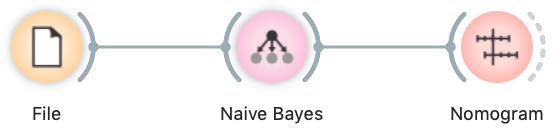
\includegraphics[scale=0.4]{workflow.png}
\end{figure}

We inspect naive Bayes models with the \widget{Nomogram} widget. There, we see a scale 'Points' and scales for each feature. Below we can see probabilities. Note the 'Target class' in upper left corner. If it is set to 'yes', the widget will show the probability that a passenger survived.

The nomogram shows that gender was the most important feature for survival. If we move the blue dot to 'female', the survival probability increases to 73\%. Furthermore, if that woman also travelled in the first class, she survived with probability of 90\%. The bottom scales show the conversion from feature contributions to probability.

\begin{figure}[h]
    \centering
    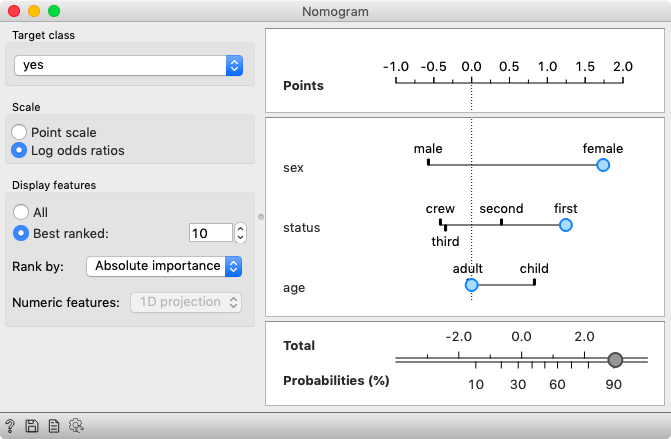
\includegraphics[scale=0.45]{nomogram.png}
    \caption{According to the probability theory individual contributions should be multiplied. Nomograms get around this by working in a log-space: a sum in the log-space is equivalent to multiplication in the original space. Therefore nomograms sum contributions (in the log-space) of all feature values and then convert them back to probability.}
\end{figure}
